\chapter{Ray-tracing model}\label{app:ray_tracing_model}

A ray-tracing model of the Technical University of Denmark have been during the processes related to this dissemination been developed. The ray-tracing model have been implemented following the details as most described in Section \ref{sec:ray-tracing}. This includes the processes of obtaining the necessary data and ensuring it is complaint with modern ray-tracing engines. Remcom Wireless Insite have been used for the ray-tracing engine, by importing a variety of data sources a full 3D model can be constructed. The software uses full 3D ray-propagation techniques accelerated by \gls{gpu}.

The obtained ray-tracing model have been used for published research papers, in particular the work found in \cite{Thrane2019ComparisonGHz, Thrane020ModelAidedDeepLearning, Thrane2020DeepKnowledge}.

\section{Data sources}

The processes for construcing the 3D polygons consisted of a relatively simple procedure using the available \gls{lidar} scans \cite{kortforsyningen}. By common practice, two scans are available, a so-called \gls{dtm} and \gls{dsm}. The former is processed to contain only height information of the terrain, while the latter contains all altitude information thus including buildings. Open-source \gls{gis} software suites such as QGIS \cite{QGISDevelopmentTeam2020QGISSystem} was used for processing the \gls{lidar} scans and zonal descriptions. The process can be described as follows. 
\begin{enumerate}
    \item Import \gls{dtm} \gls{lidar} data into QGIS as a \texttt{.geotiff} file. Ensure the coordinate reference system of the files is respected.
    \item Import \gls{dsm} \gls{lidar} data into QGIS
    \item Extract effective height. I.e. the difference between terrain height and surface height. This results in a layer with the effective height of buildings from ground level.
    \item Import zonal descriptions, i.e. building shapes and \emph{footprints} using data from \cite{OpenstreetMapWiki}.
    \item Compute and extract zonal statistics for each zone. The result is the effective heights for all building.
\end{enumerate}

The product of the above procedure results in a 3D model that can be imported into the ray-tracing engine. The result of this can be seen on Fig. \ref{fig:raytracing_model_example}. Furthermore, the terrain information can be imported resulting in buildings being placed correctly within the 3D environment.


\section{3D model}

The complexity of the ray-tracing model is determined by the number of faces present in the environment. This is ultimately determined by 1) the polygons imported, and 2) the terrain. Doing ray-tracing for a single point is effectively a computation and determination of which  \emph{rays} and the respective path are most probable within the environment. Thus, the complexity of computation and runtime hereof is determined by the total number of faces in the environment. The statistics can be seen in Table \ref{tab:ray_prop}.

\begin{table}[]
\begin{center}
\begin{tabular}{l|l}
Reflections         & 6  \\ \hline
Diffractions        & 1  \\ \hline
Area Size           & 14 $km^2$ \\ \hline
Number of buildings & 3917 \\ \hline
Number of faces     & 16563 \\ \hline
Building material   & Concrete/Brick  \\ \hline
Material Permittivity & $4.4$ to $5.3$ F/m \\ \hline
\end{tabular}
\end{center}
\caption{Properties of the ray-tracing model implemented in Remcom.}\label{tab:ray_prop}
\vspace{-1em}
\end{table}

The positions of the measurements provided by drive tests can be imported as receiver antennas into the environment. Tools for doing so have been developed for version \emph{3.3.3} of Wireless Insite. Many of the scripts can be found in the repository associated with this dissertation.

\begin{figure}
    \centering
    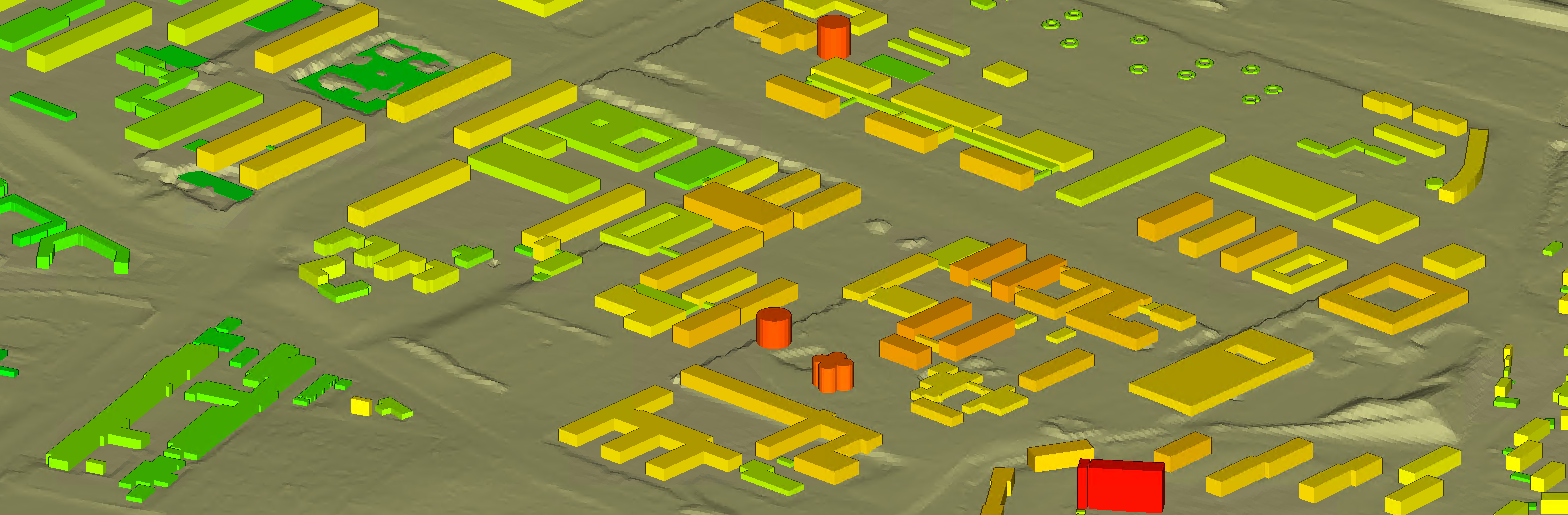
\includegraphics{appendix/figures/raytracing_3d_model_example.png}
    \caption{Screenshot from Wireless Insite with the imported 3D polygons and terrain data. Buildings are colored by height.}
    \label{fig:raytracing_model_example}
\end{figure}


%\section{Ray-tracing model calibration}


